\hypertarget{linear-block-codes}{%
\section{Linear Block Codes}\label{linear-block-codes}}

\hypertarget{channel-coding}{%
\subsection{Channel Coding}\label{channel-coding}}

\begin{itemize}
\tightlist
\item
  Channel Coding

  \begin{itemize}
  \tightlist
  \item
    Data transformations that are used for improving a system`s error
    performance
  \end{itemize}
\item
  General Idea

  \begin{itemize}
  \tightlist
  \item
    Encoder: add redundant information to the message

    \begin{itemize}
    \tightlist
    \item
      redundant: information that is already included in the message
    \item
      the transmitted data (code word) will exhibit some kind of
      structure/regularity
    \end{itemize}
  \item
    Decoder: check whether the received data still exhibit the
    prearranged structure/regularity

    \begin{itemize}
    \tightlist
    \item
      If not: An error has occurred! $\Rightarrow$ Error Detection
    \item
      Given the observed data, what is the most probable information
      that exhibits the required structure/regularity? $\Rightarrow$
      Error Correction
    \end{itemize}
  \end{itemize}
\end{itemize}

\begin{figure}[H]
\centering
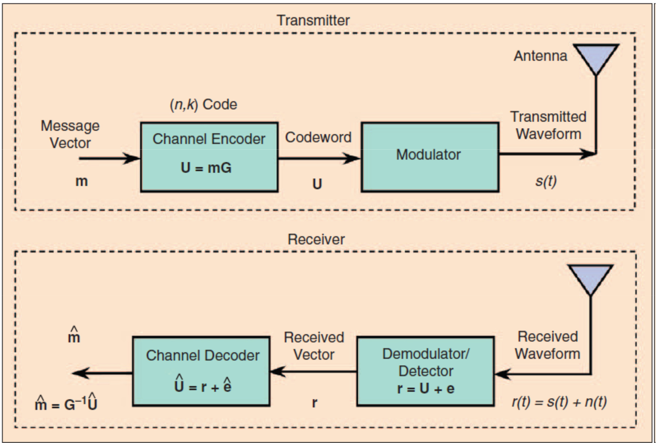
\includegraphics[width=0.6\textwidth]{figures/channelCoding.png}
\caption{Channel Coding}
\end{figure}

\clearpage
\hypertarget{nk-block-code}{%
\subsection{(n,k)-Block Code}\label{nk-block-code}}

Haben immer eine konstante Länge. Codewort hat die Länge $n$,
Nachrichtenwert hat die Länge $k$.

\begin{itemize}
\tightlist
\item
  Message block

  \begin{itemize}
  \tightlist
  \item
    consists of $k$ information symbols (from a finite field)
  \item
    $m = (m_1 , m_2 , \ldots{}, m_k )$
  \end{itemize}
\item
  Code word

  \begin{itemize}
  \tightlist
  \item
    consists of $n$ code symbols (from a finite field)
  \item
    $u = (u_1 , u_2 , \ldots{}, u_n)$
  \end{itemize}
\item
  Symbols

  \begin{itemize}
  \tightlist
  \item
    Simplest finite field: $F_2 = GF(2) \Rightarrow$ Binary Code
  \item
    also possible: $GF(2^n)$

    \begin{itemize}
    \tightlist
    \item
      binary vectors of length $n$
    \end{itemize}
  \end{itemize}
\end{itemize}

\hypertarget{hard-decisions-and-soft-decisions}{%
\subsection{Hard Decisions and Soft
Decisions}\label{hard-decisions-and-soft-decisions}}

\textbf{Demodulator}
\begin{itemize}
    \item observes the received signal r(t)
    \item produces information about the received vector $r = (r_1 , r_2 , \ldots{}, r_n )$
\end{itemize}

\textbf{Hard Decision}

\begin{itemize}
\tightlist
\item
  binary decisions, Harte Entscheidung , null oder eins
\end{itemize}

\textbf{Soft Decision}

\begin{itemize}
\tightlist
\item
  several levels of confidence

  \begin{itemize}
  \tightlist
  \item
    ``I am pretty certain, that this symbol was a 0''
  \item
    ``This symbol might be either a 0 or a 1''
  \end{itemize}
\item
  In general: better than hard decision
\end{itemize}

\hypertarget{even-parity-code}{%
\subsection{Even Parity Code}\label{even-parity-code}}

Im Prinzip eine Bitweise Exklusiv-Oder Verknüfpung mit der ganzen
Nachricht. Die Anzahl Bits muss schlussendlich gerade sein.

\begin{figure}[H]
\centering
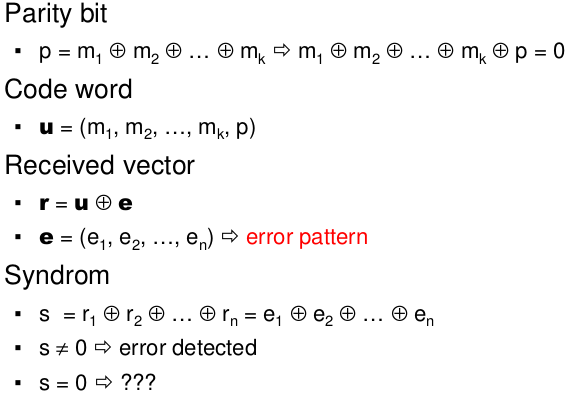
\includegraphics[width=0.5\textwidth]{figures/parityBit.png}
\caption{Even Parity Code}
\end{figure}

Falls die Prüfgleichung bzw. das Syndrom $s$ nicht erfüllt ist, bin ich
100\% sicher, dass ein Fehler aufgetreten ist. Falls $s$ 0 ergibt, haben
wir ein gültiges Code-Wort erhalten, wir wissen zwar nicht ob dies das
richtige Code-Wort ist.

\hypertarget{two-dimensional-parity-code}{%
\subsection{Two-dimensional Parity
Code}\label{two-dimensional-parity-code}}

Ich fordere über die Zeile und über die Spalte eine gerade Anzahl
Einsen. Mit diesem Code kann ich alle Einzel-Bit-Fehler korrigieren.

\begin{figure}[H]
\centering
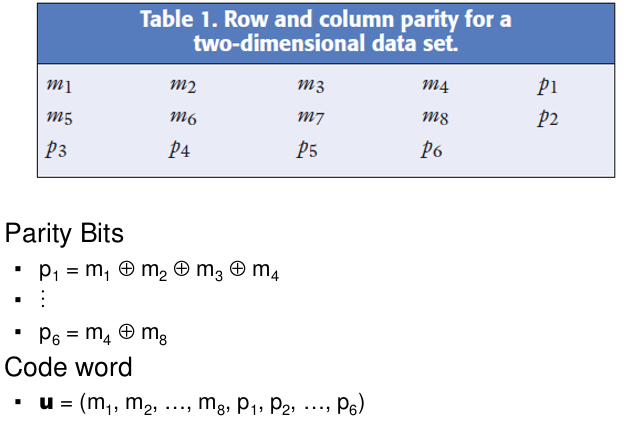
\includegraphics[width=0.5\textwidth]{figures/twoDimensionalParityCode.png}
\caption{Two-Dimensional parity code}
\end{figure}

\hypertarget{binary-linear-block-codes}{%
\subsection{Binary Linear Block Codes}\label{binary-linear-block-codes}}

\begin{tcolorbox}[colback=red!5!white,colframe=red!75!black]
A binary block code with $2^k$ code words of length $n$ is called a linear (n,k) code, if and only if its $2^k$ code words form a k-dimensional subspace of the vector space of all the n-tuples over the field $GF(2)$.
\end{tcolorbox}

\hypertarget{vector-space}{%
\subsubsection{Vector Space}\label{vector-space}}

Was ist ein Vektorraum?

\begin{itemize}
\tightlist
\item
  Eine Menge von Vektoren (Können Funktionen, normale Vektoren, egal
  sein)
\item
  Eine Menge von Skalaren (Hochgestochener Begriff für Zahlen)
\item
  Mit diesen zwei Mengen müssen folgende Operationen definiert werden:
  \begin{itemize}
  \tightlist
  \item
    Addition
  \item
    Multiplikation
  \item
    Diese beiden Operationen müssen eine Menge von Bedingungen erfüllen.
  \end{itemize}
\end{itemize}

\textbf{Beispiel}

\begin{itemize}
\tightlist
\item
  Die Menge der Skalaren ist 0 oder 1 (binäre Zahlen)
\item
  Die Menge der Vektoren sind die binären Vektoren der Länge n
\end{itemize}

\begin{figure}[H]
\centering
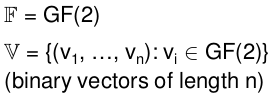
\includegraphics[width=0.3\textwidth]{figures/vektorraumBeispiel.png}
\caption{Beispiel}
\end{figure}

\hypertarget{sub-space}{%
\subsubsection{Sub Space}\label{sub-space}}

\begin{itemize}
\tightlist
\item
  Ein Vektorraum ist gegeben
\item
  Ein Unterraum ist ein Raum innerhalb des gegebenen Vektorraums
\item
  Der Unterraum ist nur ein Unterraum des Vektorraums, wenn folgende
  Bedingungen bewiesen werden können.
\end{itemize}

\begin{figure}[H]
\centering
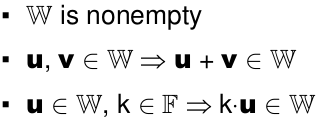
\includegraphics[width=0.3\textwidth]{figures/subspaceRequirements.png}
\caption{Bedingungen}
\end{figure}

\hypertarget{linear-combination}{%
\subsection{Linear Combination}\label{linear-combination}}

\begin{itemize}
\tightlist
\item
  Gegeben sind Skalare $a$ und Vektoren $v$
\item
  Durch die Kombination von einbisschen $v_1 * a_1 + v_2 * a_2$ usw. ergibt
  sich eine Linearkombination.
\item
  Das Set von allen möglichen Linearkombinationen ergibt ein Unterraum
  von $V$.
\item
  Wenn die Vektoren Linear unabhängig sind (sie zeigen nicht in die
  gleiche Richtung), kann ich mit $k$ Vektoren einen Unterraum mit der
  Dimension $k$ erstellen.
\end{itemize}

\begin{figure}[H]
\centering
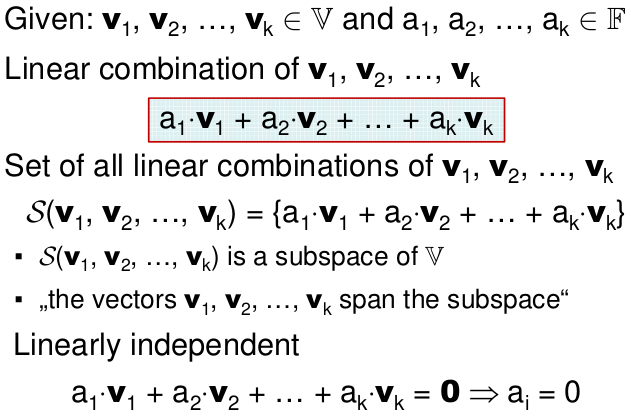
\includegraphics[width=0.5\textwidth]{figures/linearKombination.png}
\caption{Linear Combination}
\end{figure}

\hypertarget{generator-matrix}{%
\subsubsection{Generator Matrix}\label{generator-matrix}}

\begin{itemize}
\item
  The entire vector space $V$ of binary vectors of length $n$ contains $2^n$
  elements
\item
  A linear $(n, k)$ block code is a $k$-dimensional subspace of $V$ that
  contains $2^k$ binary vectors of length $n$
\item
  It is possible to find $k$ linearly independent code words $g_1 , g_2 ,
  \ldots{} g_k$ such that every code word u is a linear combination of
  these $k$ code words
\item
  Alle lineare Kombinationen, die ich generieren bzw. schreiben kann,
  ergibt die Menge der Codewörter
\item
  Man kann den Code (Menge von Code-Wörtern) auch mit einer
  Generator-Matrix schreiben, in dem man die möglichen Code-Wörter und
  die Nachrichten als Vektoren darstellt und multipliziert
\item
  Es kann mehr also nur eine Generator-Matrix geben
\end{itemize}

\begin{figure}[H]
\centering
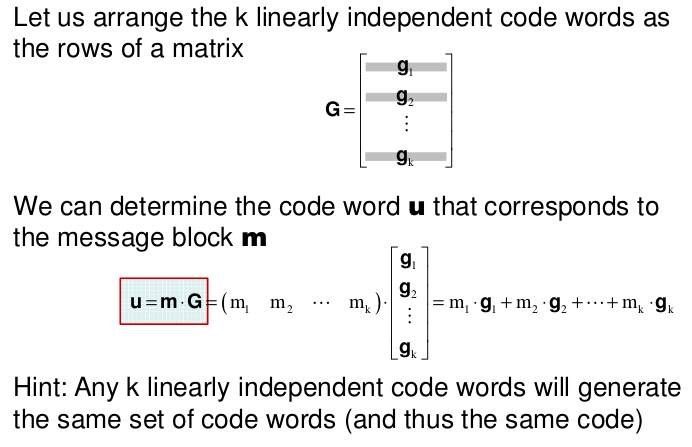
\includegraphics[width=0.6\textwidth]{figures/generatorMatrix.png}
\caption{Generator Matrix}
\end{figure}

\hypertarget{weight-and-distance-properties}{%
\subsection{Weight and Distance
Properties}\label{weight-and-distance-properties}}

\begin{itemize}
\tightlist
\item
  \textbf{Hamming Weight w(u):} Number of nonzero elements in u. Anzahl
  Einsen
\item
  \textbf{Hamming distance d(u,v):} Number of bit positions in which u
  and v differ

  \begin{itemize}
  \tightlist
  \item
    $u = (1 0 1 1 0 1)$ and $v = (0 0 1 1 1 1) \Rightarrow d(u,v) = 2$
  \end{itemize}
\item
  Properties

  \begin{itemize}
  \tightlist
  \item
    $d(u,v) = w(u + v)$
  \item
    $d(u,0) = w(u)$
  \item
    $d(u,v) \leq d(u,w) + d(w,v)$
  \end{itemize}
\item
  \textbf{Minimum Hamming weight of a code}

  \begin{itemize}
  \tightlist
  \item
    Jedes Gewicht der einzelnen Code-Wörtern miteinander vergleichen
  \item
    $w_{min}(C) = min \{w(u): u \in C, u \neq 0\}$
  \end{itemize}
\item
  \textbf{Minimum Hamming distance of a code C}

  \begin{itemize}
  \tightlist
  \item
    Dazu muss ich jedes einzelne Code Wort nehmen und die
    Hamming-Distanz zu v ausrechnen und dann mit allen anderen möglichen
    Distanzen vergleichen.
  \item
    $d_{min}(C) = min \{d(u,v): u,v \in C, u \neq v\}$
  \end{itemize}
\end{itemize}

\begin{tcolorbox}[colback=red!5!white,colframe=red!75!black]
The minimum distance of a linear block code is equal to the minimum weight of its nonzero code words
\end{tcolorbox}

\hypertarget{decoding}{%
\subsection{Decoding}\label{decoding}}

\begin{itemize}
\tightlist
\item
  Ich probiere jedes Code-Wort $u$, das gesendet werden kann durch und
  berechne die Wahrscheinlichkeit, ob das Empfangene $r$ tatsächlich zum
  Code-Wort passt
\item
  Das Code-Wort $u$, das die höchste Wahrscheinlichkeit hat, nehme ich
\end{itemize}

\begin{figure}[H]
\centering
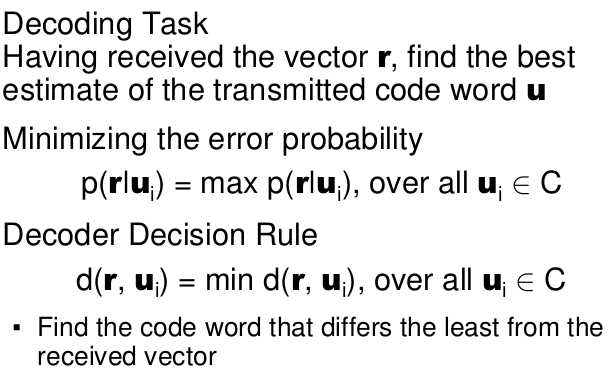
\includegraphics[width=0.5\textwidth]{figures/decoding.png}
\caption{Decoding}
\end{figure}

\begin{figure}[H]
\centering
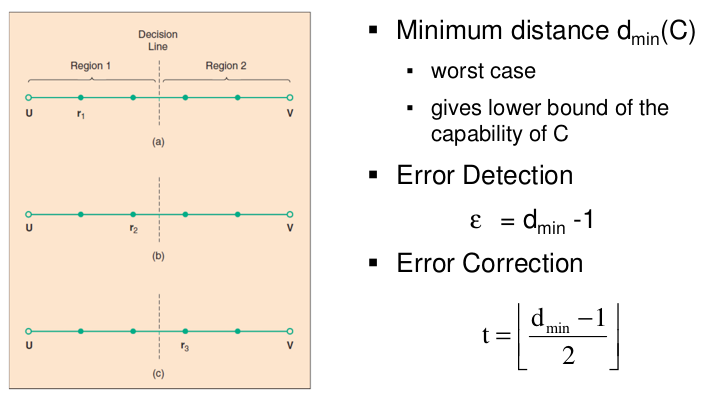
\includegraphics[width=0.5\textwidth]{figures/detecting.png}
\caption{Detecting and Correction}
\end{figure}

\begin{figure}[H]
\centering
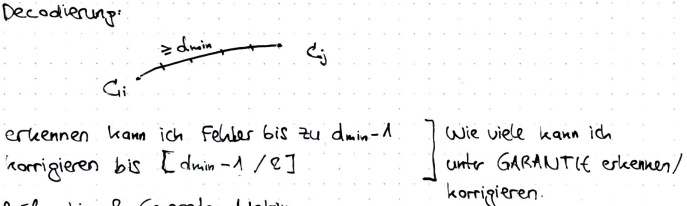
\includegraphics[width=0.8\textwidth]{figures/notesDecoding.png}
\caption{Notes Decoding}
\end{figure}

\hypertarget{example}{%
\subsection{Example}\label{example}}

\begin{figure}[H]
\centering
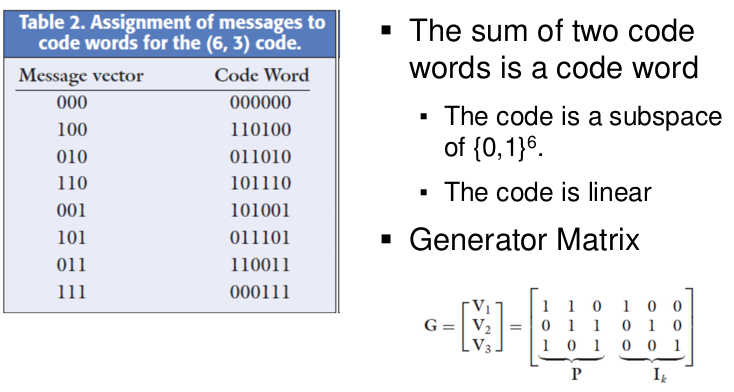
\includegraphics[width=0.5\textwidth]{figures/63blockCode.png}
\caption{Example}
\end{figure}

\begin{itemize}
\tightlist
\item
  Der Block Code ist linear, da jede Operation zweier Code Wörter immer
  wieder ein valides Code Wort ergeben
\item
  Darum gibt es auch eine generator Matrix
\item
  Es ist offensichtlich, dass die drei Zeilen in $G$ linear unabhängig
  sind, da der Block $I$ eine Einheitsmatrix ist.
\item
  Wenn wir die Tabelle mit den möglichen Code-Wörtern haben und die
  Aufgabe haben, eine mögliche Generator Matrix zu finden, dann besteht
  die Aufgabe einzig und allein darin, $k$ (in unserem Fall 3) mögliche
  unabhängige Codewörter zu finden.
\end{itemize}

\hypertarget{parity-check-matrix-oder-pruxfcf-matrix}{%
\subsection{Parity Check Matrix (oder Prüf
Matrix)}\label{parity-check-matrix-oder-pruxfcf-matrix}}

\begin{itemize}
\tightlist
\item
  $u$ ist ein gültiges Code-Wort, wenn $u * H^T = 0$ ist
\item
  $H$ ist die Prüfmatrix
\end{itemize}

\begin{figure}[H]
\centering
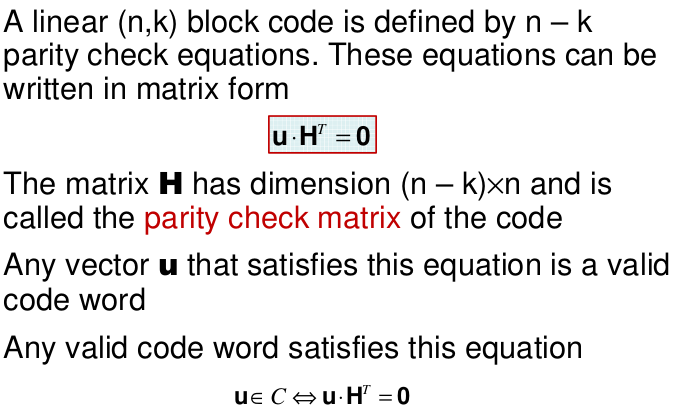
\includegraphics[width=0.5\textwidth]{figures/pruefmatrix.png}
\caption{PruefMatrix}
\end{figure}

\begin{figure}[H]
\centering
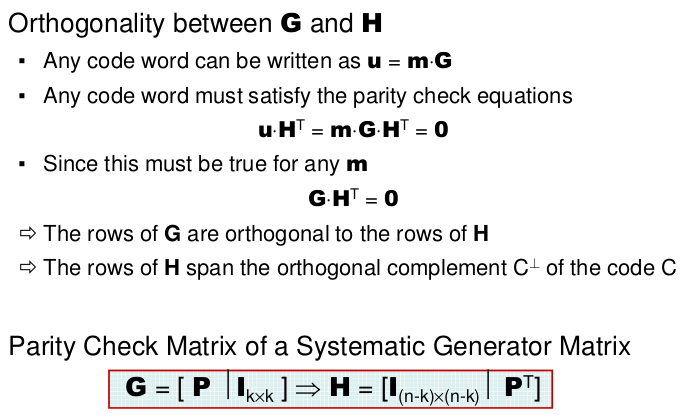
\includegraphics[width=0.5\textwidth]{figures/BeziehungGundH.png}
\caption{Relation G and H}
\end{figure}

\begin{itemize}
\tightlist
\item
  $m$ ist immer ein gültiges Code-Wort, daher muss $m*G*H^T$ immer 0
  ergeben
\item
  Das bedeutet nur, dass die Zeilen von $G$ und die Spalten von $H^T$
  orthogonal zueinander stehen
\item
  Für den Fall, dass die Generator Matrix Systematisch ist (sie hat im
  hinteren Teil eine Einheitsmatrix), kann ich aus dieser ganz einfach
  eine Prüfmatrix erstellen
\end{itemize}

\hypertarget{syndrom-testing}{%
\subsection{Syndrom Testing}\label{syndrom-testing}}

\begin{itemize}
\tightlist
\item
  Um zu prüfen, ob der erhaltene Vektor $r$ ein valider Code ist, kann man das Syndrom bilden.
\item
  Ist das Syndrom $0$, so ist der erhaltene Code valid
\item
  Ist das Syndrom nicht $0$, so kann aus dem Syndrom der entsprechende
  Fehler herausgefunden werden
\end{itemize}

\begin{figure}[H]
\centering
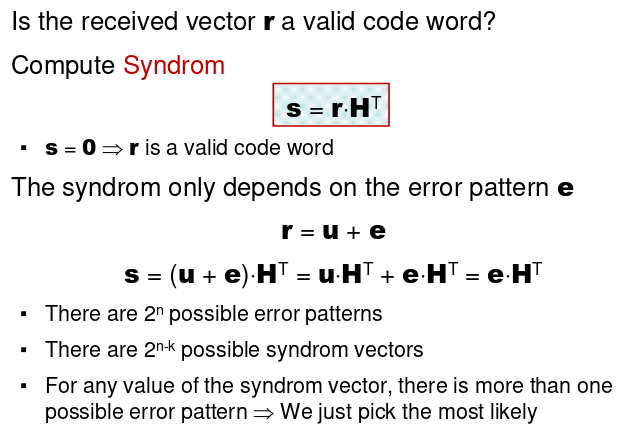
\includegraphics[width=0.5\textwidth]{figures/syndromTesting.png}
\caption{Syndrom Testing}
\end{figure}

\begin{figure}[H]
\centering
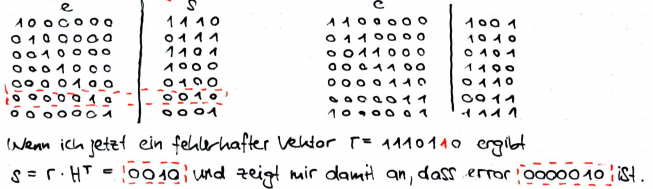
\includegraphics[width=0.8\textwidth]{figures/syndromTestingNotes.png}
\caption{Notes Syndrom Testing}
\end{figure}

\subsection{Decoder}
\begin{figure}[H]
\centering
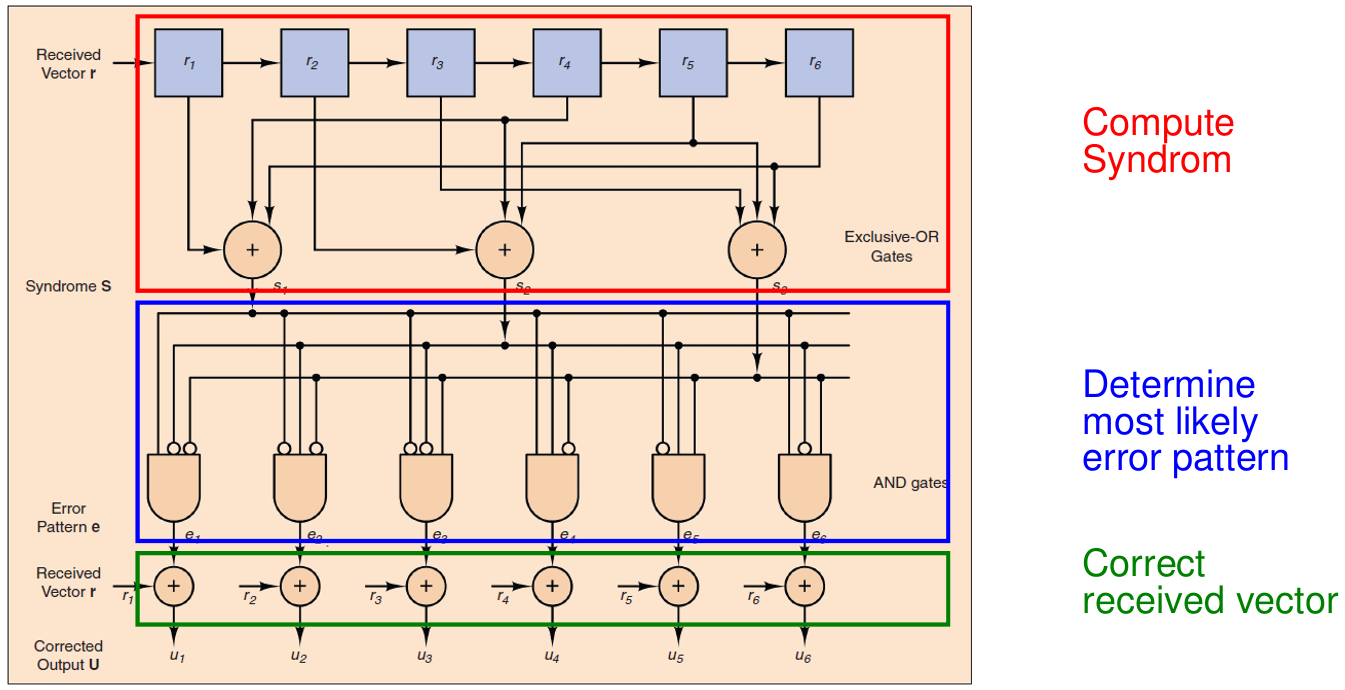
\includegraphics[width=0.6\textwidth]{figures/lbc_decoder.png}
\caption{LCB - Decoder}
\end{figure}

\begin{itemize}
    \item Rot: Aus dem empfangenen Vektor wird das Syndrom (Resultate der drei Prüfgleichungen) berechnet.
    \item Blau: Syndromtabelle. Input ist der Wert des Syndroms, Output ist das wahrscheinlichste Fehlermuster.
    \item Grün: Korrektur des empfangenen Vektors mit dem zuvor ermittelten Fehlermuster.
\end{itemize}

\subsection{Cyclic Codes}
 Jeder zyklische Code ist ein linearer Blockcode (es gibt eine Generatormatrix, Prüfmatrix und die Kombination von Codes ergibt wieder einen Code).\\

\textbf{Die neue Eigenschaft:}
Jedes Codewort kann zyklisch verschoben werden (bit shift), was wieder ein Codewort ergibt.\\

Repräsentation eines binären Vektors (Codewort) als Polynom.
X ist ein Platzhalter (Funktion von X).

\begin{figure}[H]
\centering
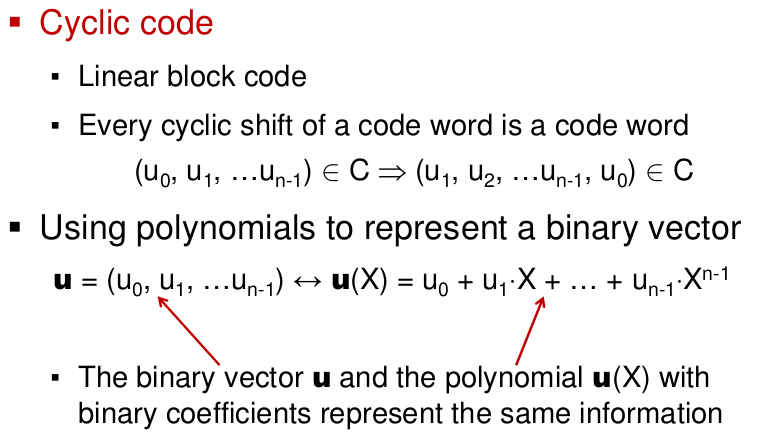
\includegraphics[width=0.5\textwidth]{figures/cyclic_codes.png}
\caption{Cyclic Codes}
\end{figure}

\subsection{Generator Polynom}
In jedem zyklischen Code gibt es genau ein Codewort, dessen Polynomdarstellung exakt den Grad $n-k$ besitzt und $g_0 = 1$ ist. $\Rightarrow$ Das ist das Generatorpolynom. \\

Wenn ein Vektor ein Codewort ist, muss dessen Polynomdarstellung ein vielfaches des Generatorpolynoms sein.

\begin{figure}[H]
\centering
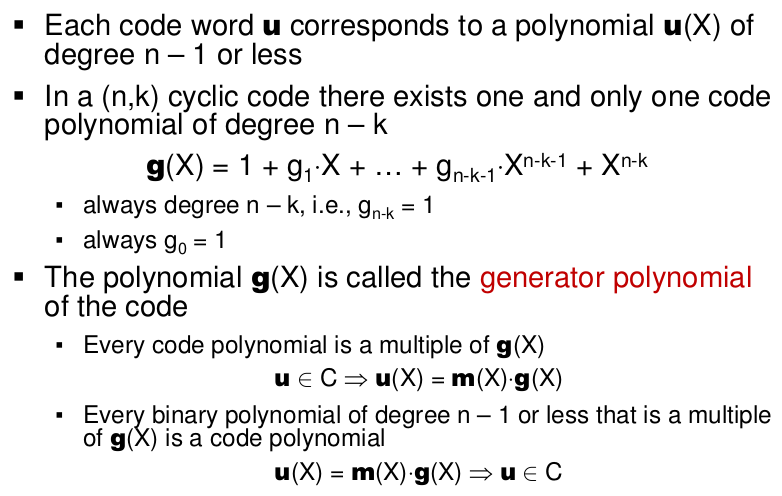
\includegraphics[width=0.5\textwidth]{figures/generator_polynom.png}
\caption{Generator Polynom}
\end{figure}

\subsection{Systematic Cyclic Codes}
Das zuvor beschriebene Verfahren resultiert in einem nicht systematischen Codewort (die Nachrichten-Bits erscheinen nicht im Codewort).Nun möchten wir ein systematisches Codewort erhalten, in dem am Ende des Codewortes die Nachrichten-Bits vorkommen.

Wandelt man dieses Format in ein Polynom $u(X)$ um, erhält man das Polynom der Nachricht multipliziert mit  addiert mit den Prüfbits. Damit das Ganze ein Codewort ist, muss $u(X)$ ein Vielfaches des Generatorpolynoms sein.

Wir müssen also $p(X)$ so wählen, dass dies erfüllt ist (roter Kasten).
Man berechnet also $p(x)$ und verkettet das mit der Nachricht.

Daraus erhält man ein systematisches Codewort.

\begin{figure}[H]
\centering
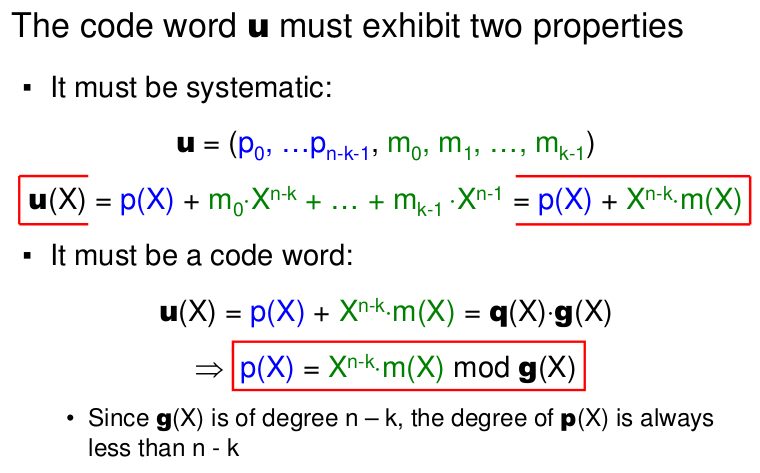
\includegraphics[width=0.5\textwidth]{figures/systematic_cyclic_codes.png}
\caption{Systematic Cyclic Codes}
\end{figure}

\subsection{Linear Shift Registers}
Ein Vorteil von zyklischen Codes ist, dass Encoder und Decoder einfach gebaut werden können.
Der Input (unten) sind die Nachrichtenbits. Oben sind linear rückgekoppelte Schieberegister mit den Termen des Generatorpolynoms. Das Register dividiert durch $g(x)$. Sobald alle Nachrichtenbits durchgegeben wurden, schaltet der Schalter 2 um. Der Output ist dann der Rest der Division (die $n-k$ Prüfbits $p(X)$).

\begin{figure}[H]
\centering
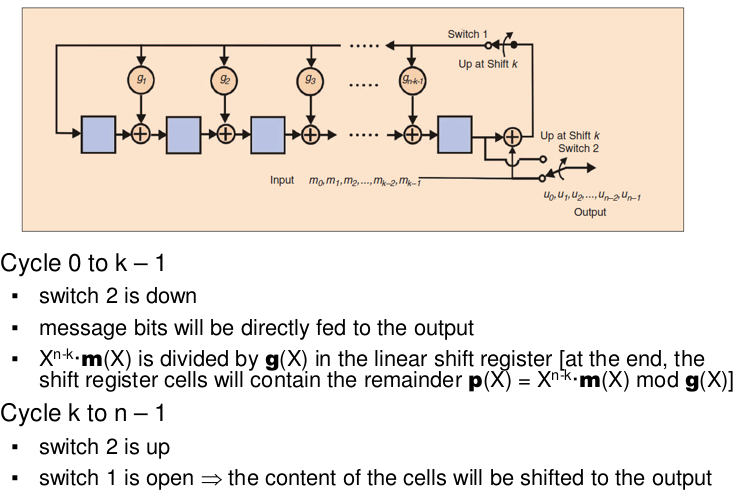
\includegraphics[width=0.5\textwidth]{figures/linearShiftRegister.png}
\caption{Linear Shift Register}
\end{figure}

\begin{figure}[H]
\centering
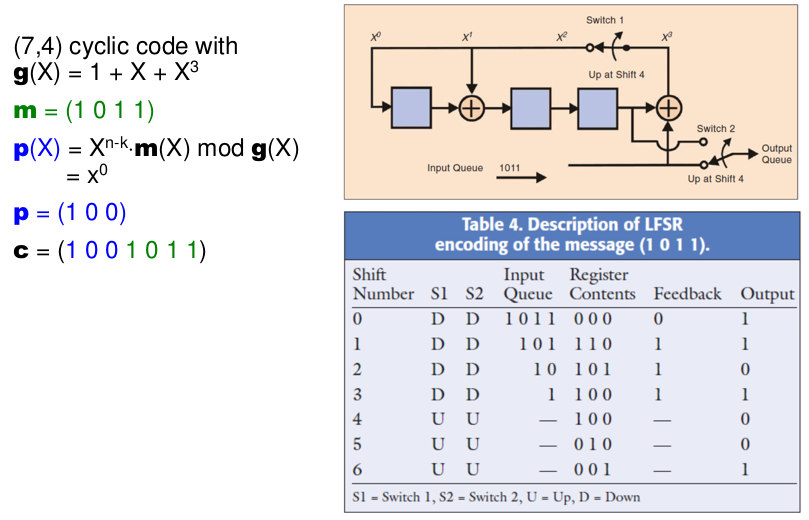
\includegraphics[width=0.5\textwidth]{figures/linearShiftRegisterExample.png}
\caption{Linear Shift Register - Example}
\end{figure}

\subsection{Error Correction}
Korrektur funktioniert ähnlich zu linearen Codes.
\begin{itemize}
    \item Ein Codewort muss restlos durch das Generatorpolynom dividierbar sein (weil es ein Vielfaches dessen ist).
    \item Der Rest der Division nennt man das Syndrompolynom.
    \item Ist das Syndrompolynom = 0 ist es ein gültiges Codewort.
    \item Ist das Syndrompolynom nicht = 0, gab es einen Fehler.
    \item Das Syndrompolynom hängt also wie auch bei linearen Codes nur vom Fehlermuster ab.
    \item Man erzeugt analog auch eine Syndromtabelle und bestimmt das "wahrscheinlichste" Codewort aus dem Fehlermuster (Syndrompolynom).
\end{itemize}


\clearpage